\begin{figure}[h!]
    \centering
    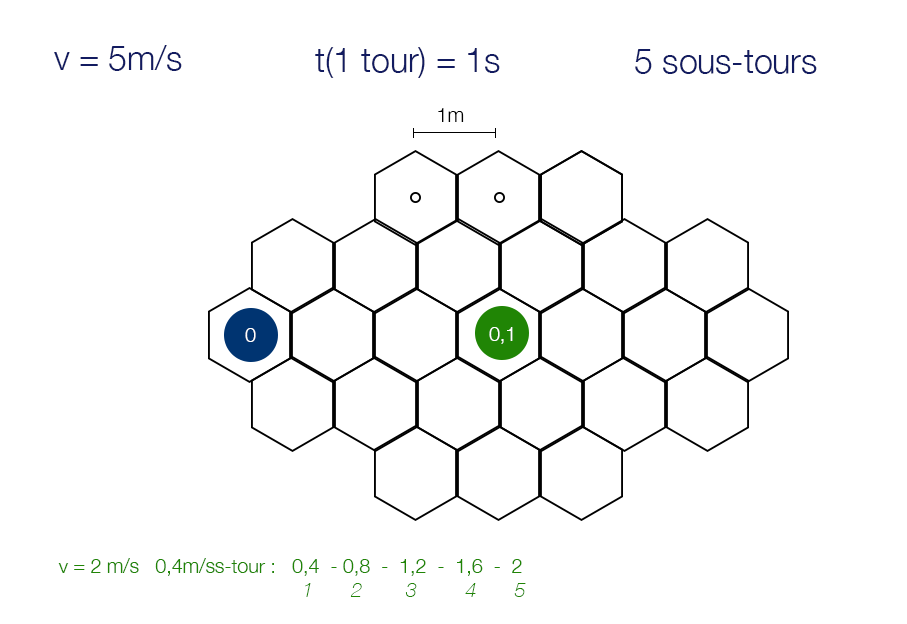
\includegraphics[width=0.3\textwidth]{../TurnModel/TurnModel0.png}
    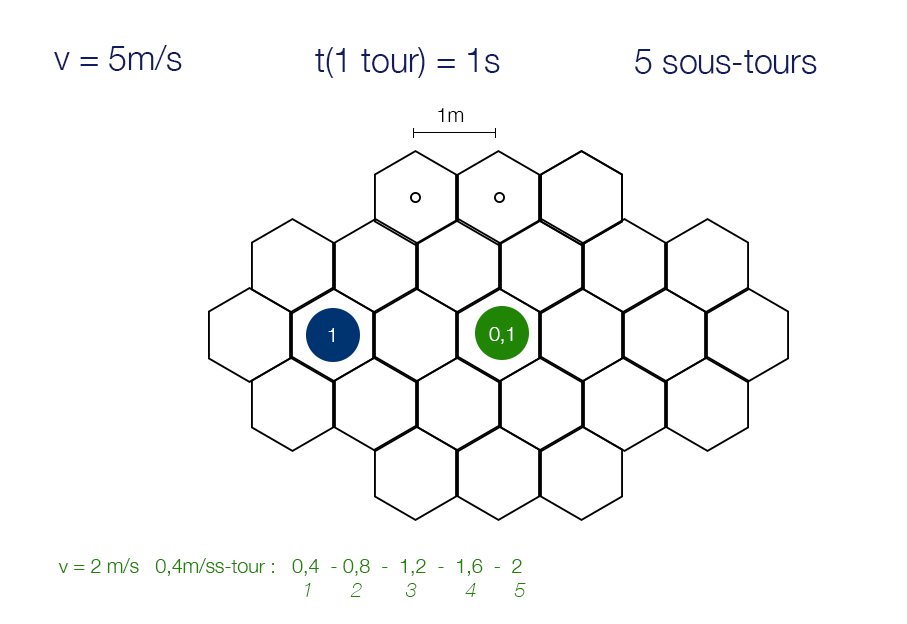
\includegraphics[width=0.3\textwidth]{../TurnModel/TurnModel1.png}
    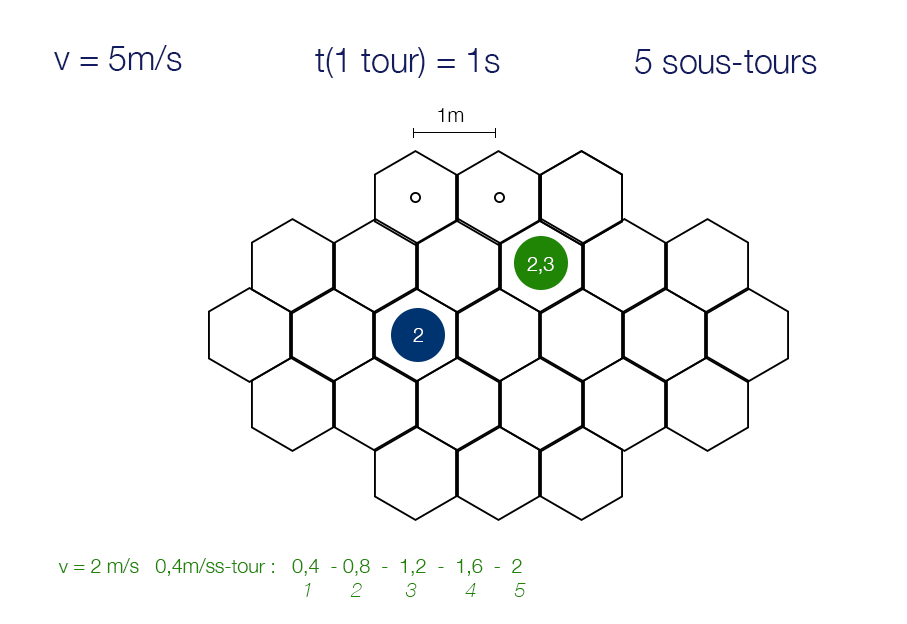
\includegraphics[width=0.3\textwidth]{../TurnModel/TurnModel2.png}
    \\
    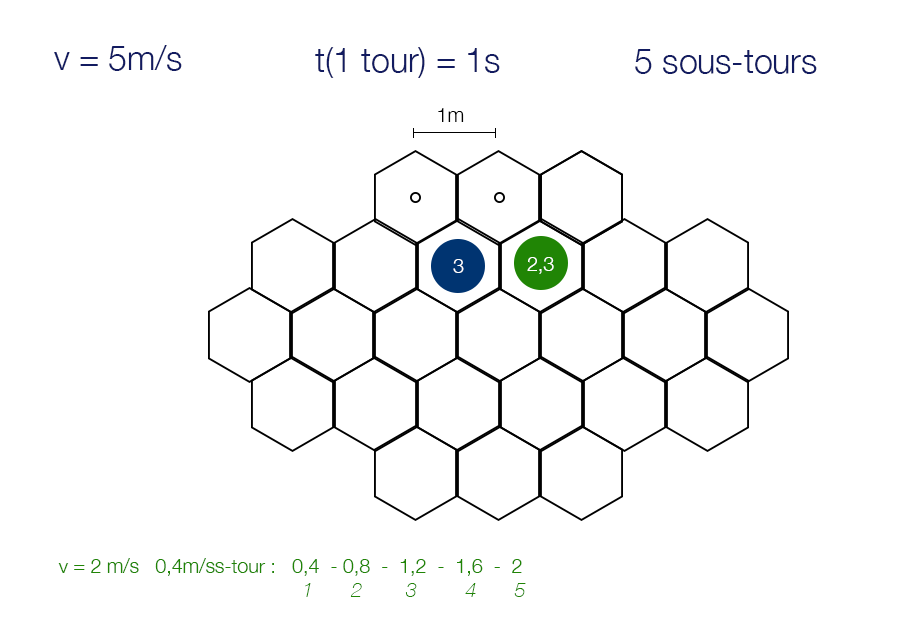
\includegraphics[width=0.3\textwidth]{../TurnModel/TurnModel3.png}
    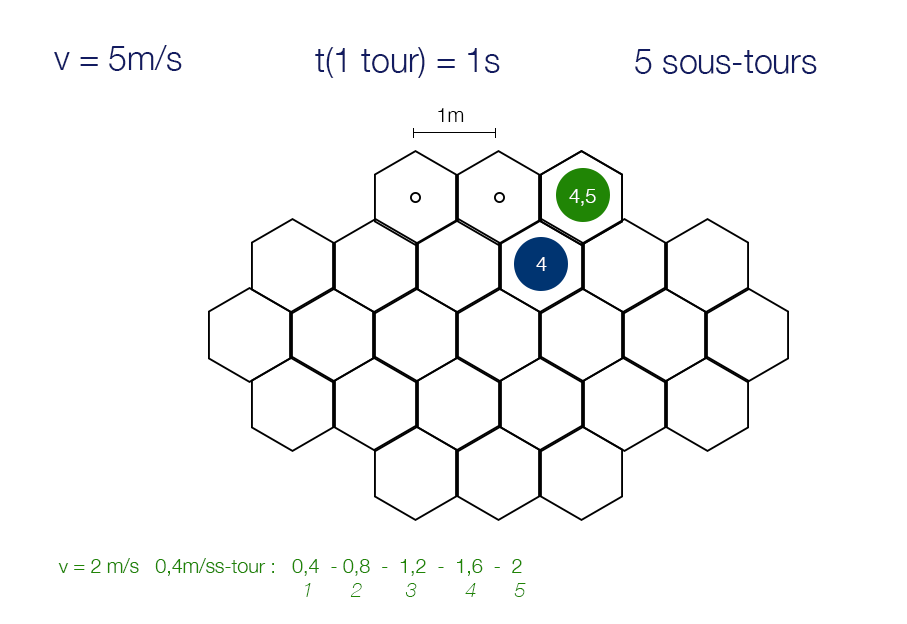
\includegraphics[width=0.3\textwidth]{../TurnModel/TurnModel4.png}
    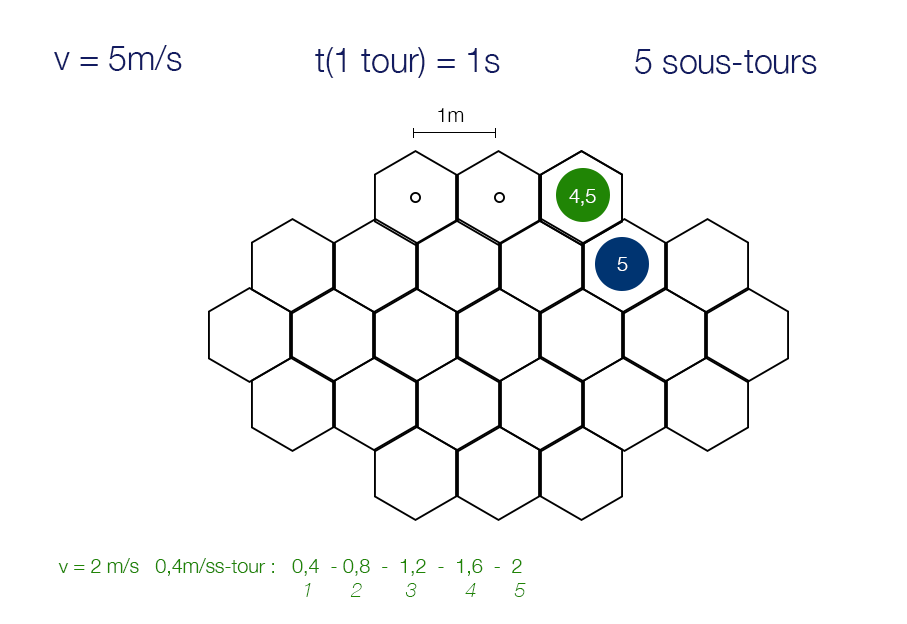
\includegraphics[width=0.3\textwidth]{../TurnModel/TurnModel5.png}
    \caption{\label{fig:TurnModel} Déplacements des joueurs sur le terrain}
\end{figure}

\subsection{Terrain}
Figure \ref{fig:TurnModel}

Un terrain de Quidditch est délimité par un ovale, et est constitué de cases hexagonales de 10 pieds\footnote{3.048 m}. Il fait 50 cases dans sa plus grande longueur, et 18 cases dans sa plus grande largeur, pour un total de 706 cases sur le terrain.

Chaque case ne peut accueillir qu'un seul joueur au maximum. Si deux joueurs arrivent au même tour sur la même case, une collision a lieu. Selon les \gls{aptitude}s et les rôles des joueurs, différentes actions indirectes pourront avoir lieu.
